
\section{Introduction and Motivation}

 TODO: re-enable on long paper
Exploring long term alternatives to the CMOS technology is gaining
more and more revelance as the scaling trend of such devices keeps
introducing new challenges. Power density, defect tolerance, testing
costs and wire delays are only a few of the many critical aspects
involved~\cite{itrs12}. While software parallelism and multicore
approaches~\cite{horowitz2004, mudge2001, powell2009} are partially mitigating the impact of such
constraints on performances, it is likely that the growing computing demand will
eventually need even more radical architectural modifications and new
paradigms in order to address the Computer Design challenges of the next
decades.

In the last years, Self-assembled nanoscale architectures~\cite{winfree1998, yan2003}
are emerging as a promising technology due their tera/peta scale of
integration, defect tolerance and huge potential computing
capabilities. These technologies are certainly still at
their early stage of development, however different laboratory demos and
prof-of-concepts architectures have been presented~\cite{patwardhan2004, patwardhan2006_1, pistol2009}.
%, patwardhan2006
The main idea behind this approach is to exploit the physical regularity and
stability of DNA structures in order to create a scaffold onto which
nano-devices (e.g. nanowires and CNFETs~\cite{bachtold2001, tans1998, cui2001}) can be
attached. This can be achieved by designing appropriate complementary DNA tags for
each terminal to be placed, so that a nano device will be attached
only where its own DNA tag matches a complementary tag on the DNA grid
scaffold.
A detailed description of the chemical properties involved is far
beyond the scope of this paper (see also~\cite{braun1998, seeman1999}), so we will focus on
the three main challenges that this new fabrication process introduces
in Computer Design: \emph{(i) limited node complexity}, \emph{(ii) large scale
randomness} and \emph{(iii) high defect rates}.  

The \emph{limited node complexity} aspect is directly
related to the use of complementary DNA tags in order to place circuit
components. In a traditional CMOS process the complexity is introduced
using a photolithography mask, so that larger (more complex) circuits
only require larger masks; conversely, self-assembly achieves
complexity by increasing the number of unique DNA tags, since more
different tags means having more control on component placement. Ideally, by specifying a single
and unique tag for each nano transistor terminal, we could exactly
choose where each component would be placed. But the number of DNA
symbols forming the DNA sequence is limited (sequence of 4 nucleobases
G,A,T,C) and so creating many different tags (of a given lenght) would
mean make them more similar to each other, increasing the probability
of incorrect/partial matching. To avoid this problem we should limit
the number of unique tags, thus limiting the complexity at each node.
In particular, a budget of about $10,000$ CNFETs per node has been
estimated in~\cite{liu_jetcs}.

\emph{Large scale randomness} is the other fundamental condition of
self-assembled technology: DNA tags allow a control placement inside
node grid, but there is no control of where each of these  grids will
be placed on the whole network. As a consequence, other typical
properties of regular networks cannot be guaranteed, e.g. being
connected to a fixed number of neighbors, having a determined
orientation and so on.

Finally, \emph{defect rates}: while they are very hardly tolerated in mask
based top down design , the same nature of a bottom up self
assembled process cannot assume such a deterministic device placement
process, thus defect tolerance is something like a design requirement
more than an exception to be avoided.

\begin{figure*}
\centering
\begin{tabular}{cc}
    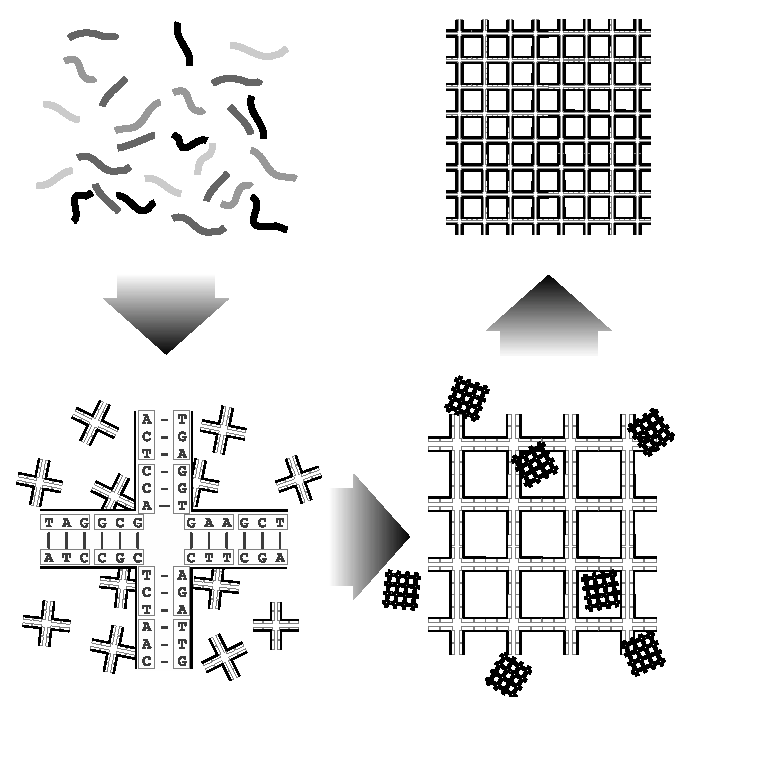
\includegraphics[width=0.40\textwidth]{pictures/dna2b.eps} &
    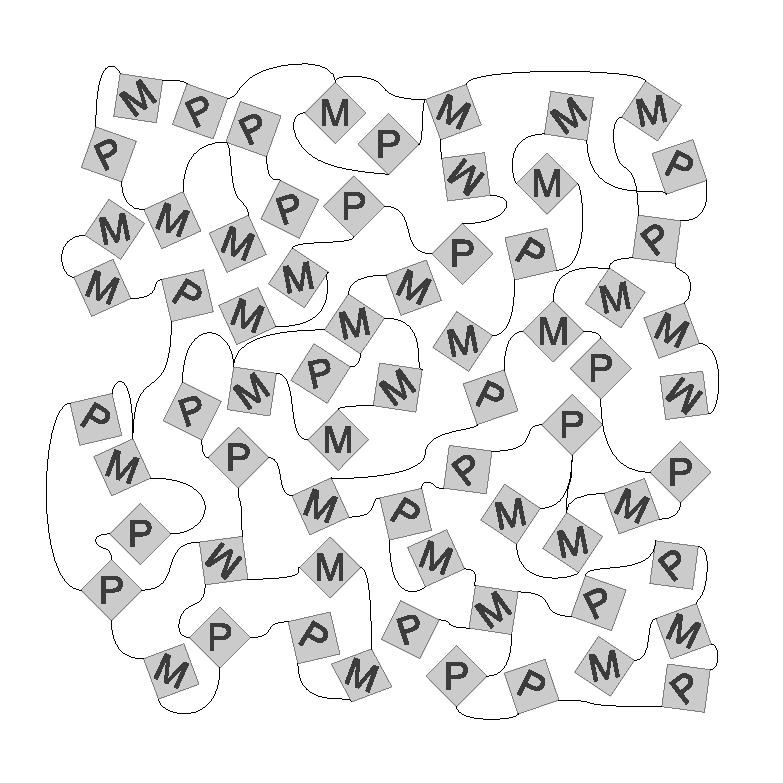
\includegraphics[width=0.40\textwidth]{pictures/dna1_complex2.eps} \\
 (a) & (b)
 \end{tabular}
  \caption{DNA tag matching and Resulting Irregualr Topology}
  \label{fig:nana}
\end{figure*}
These aspects of a DNA-self assembly process lead to some important
implications to be addressed when approaching to the design of
computer architecture: a computational model should be based on a
distributed network of small computing and storage nodes, randomly
placed and interconnected (see Figure~\ref{fig:nana}).
Proof-of-concept of such kind of computational model can be found for
example in~\cite{patwardhan2006_1}.  Since no regularity can be
assumed in such network, a topology agnostic strategy that avoids
deadlock should be adopted in order to route packets (e.g.
instructions and data operands) among nodes.  It is important to
underline that, altougth we can assume an architecture similar to the
one depicted in Figure~\ref{fig:nana} as background, the topology discovery
problem faced in this work is more general and not strictly dependent on any of the
underlying computing architecture.

In this work we introduce DiSR, a Distributed Segment-based approach
to deadlock freedom in large scale DNA self assembled networks. Our
contribution aims to achieve the classical properties of a
segment-based approach~\cite{mejia_ipdps06} without requiring any
topology graph, external defect map or centralized algorithm
execution.  So the DiSR approach is not intended to discover the
``optimal'' segment choice (ideally reachable with the knowledge of
the topology graph) but just to demonstrate a concrete model that can
fit into such complex, irregular and large sized networks.

The paper is organized as follows: in Section~\ref{sec:related_works}
we summarize the main approaches to topology agnostic routing. Next in
Section~\ref{sec:disr_concepts} are described the main elements and
the execution model of the proposed approach.  In Section~\ref{sec:simulation}
simulations are carried out with the opensource tool Nanoxim to
demonstrate how DiSR preserves some of the main segment-based
properties and how compares to the tree-based approaches. Finally a
draft of a architectural implementation is shown in
Section~\ref{sec:implementation} to evaluate the feasibility of the
approach in terms of node complexity.

\section{Related Works}
\label{sec:related_works}
Several works~\cite{sancho2002, skeie2002, skeie2004, koibuchi2003} have been presented addressing the problem of topology
agnostic routing. While they show interesting
performances, the requirement for virtual channels resources 
to avoid deadlock makes them not suitable for the specific DNA self
assembled networks we are assuming as background.
Other topology independent algorithms~\cite{schroeder1991, koibuchi2001, cherkasova1996} do not use virtual channels to
achieve deadlock freedom, but turn prohibitions. 
In particular, authors of~\cite{Patwardhan05evaluatingthe} exploits the creation of a spanning tree of the
topology, then placing bidirectional restrictions by avoiding a packet
to traverse the same link in both up and down directions.
While the hierarchical nature of this approach can lead to uneven traffic
distribution, with many packets traversing upper links (near to the
root), this is quite acceptable in classical wide area networks
topologies with a limited number of nodes. Other approaches such as
FX~\cite{sancho2000} mitigate this
issue, but the set of turn restrictions is still prefixed,
strictly depending on the particular tree root selected. 
Other solutions try to approach the issue of irregular
topologies by limiting the number~\cite{dally1994, duato1997, gomez2004, koibuchi2008} or the
location~\cite{zhang2008, sui2000, flich2008, liu2011} of missing links. This
restriction is clearly unacceptable given the hight-defect rates of
DNA self-assembled networks scenario. For the same reason, we also
avoid considering solutions based on hardware-redundancy to
dynamically recover defects as in~\cite{constantinides2006, kohler2010, kim2006, park2006, ebrahimi2013}. 

In~\cite{mejia_ipdps06} authors present SR, an approach the solves these
limitations by allowing turn restrictions to be placed locally,
independently from other restrictions. The whole network is
partitioned into segments, and each bidirectional turn
restriction can be freely chosen within a segment in order to guarantee
deadlock freedom and connected networks. This \emph{locality
independence} property, together with no requirement of any particular tree/root
choice, would make it the best choice for the given scenario;
however, its topology independency still requires the knowledge of the
whole network graph in order to find the segments. 

The DiSR approach presented in this work is a first attempt of
reaching the same goals of a segment based approach, that is
establishing segments, without requiring any topology graph or
centralized execution. 



